\section*{Resultater}
\label{Resultater}
%
Ud fra det udarbejdede \textit{affinity diagram} udvælges de to grønne, overordnede kategorier, der er relevante i forhold til dette mini projekt, som er: \textit{Robottens udseende}, illustreret på \autoref{fig:RsUdseende}, samt \textit{Robottens væremåde}, illustreret på \autoref{fig:RsVaeremaade}.
%
\begin{figure}[H]
\centering
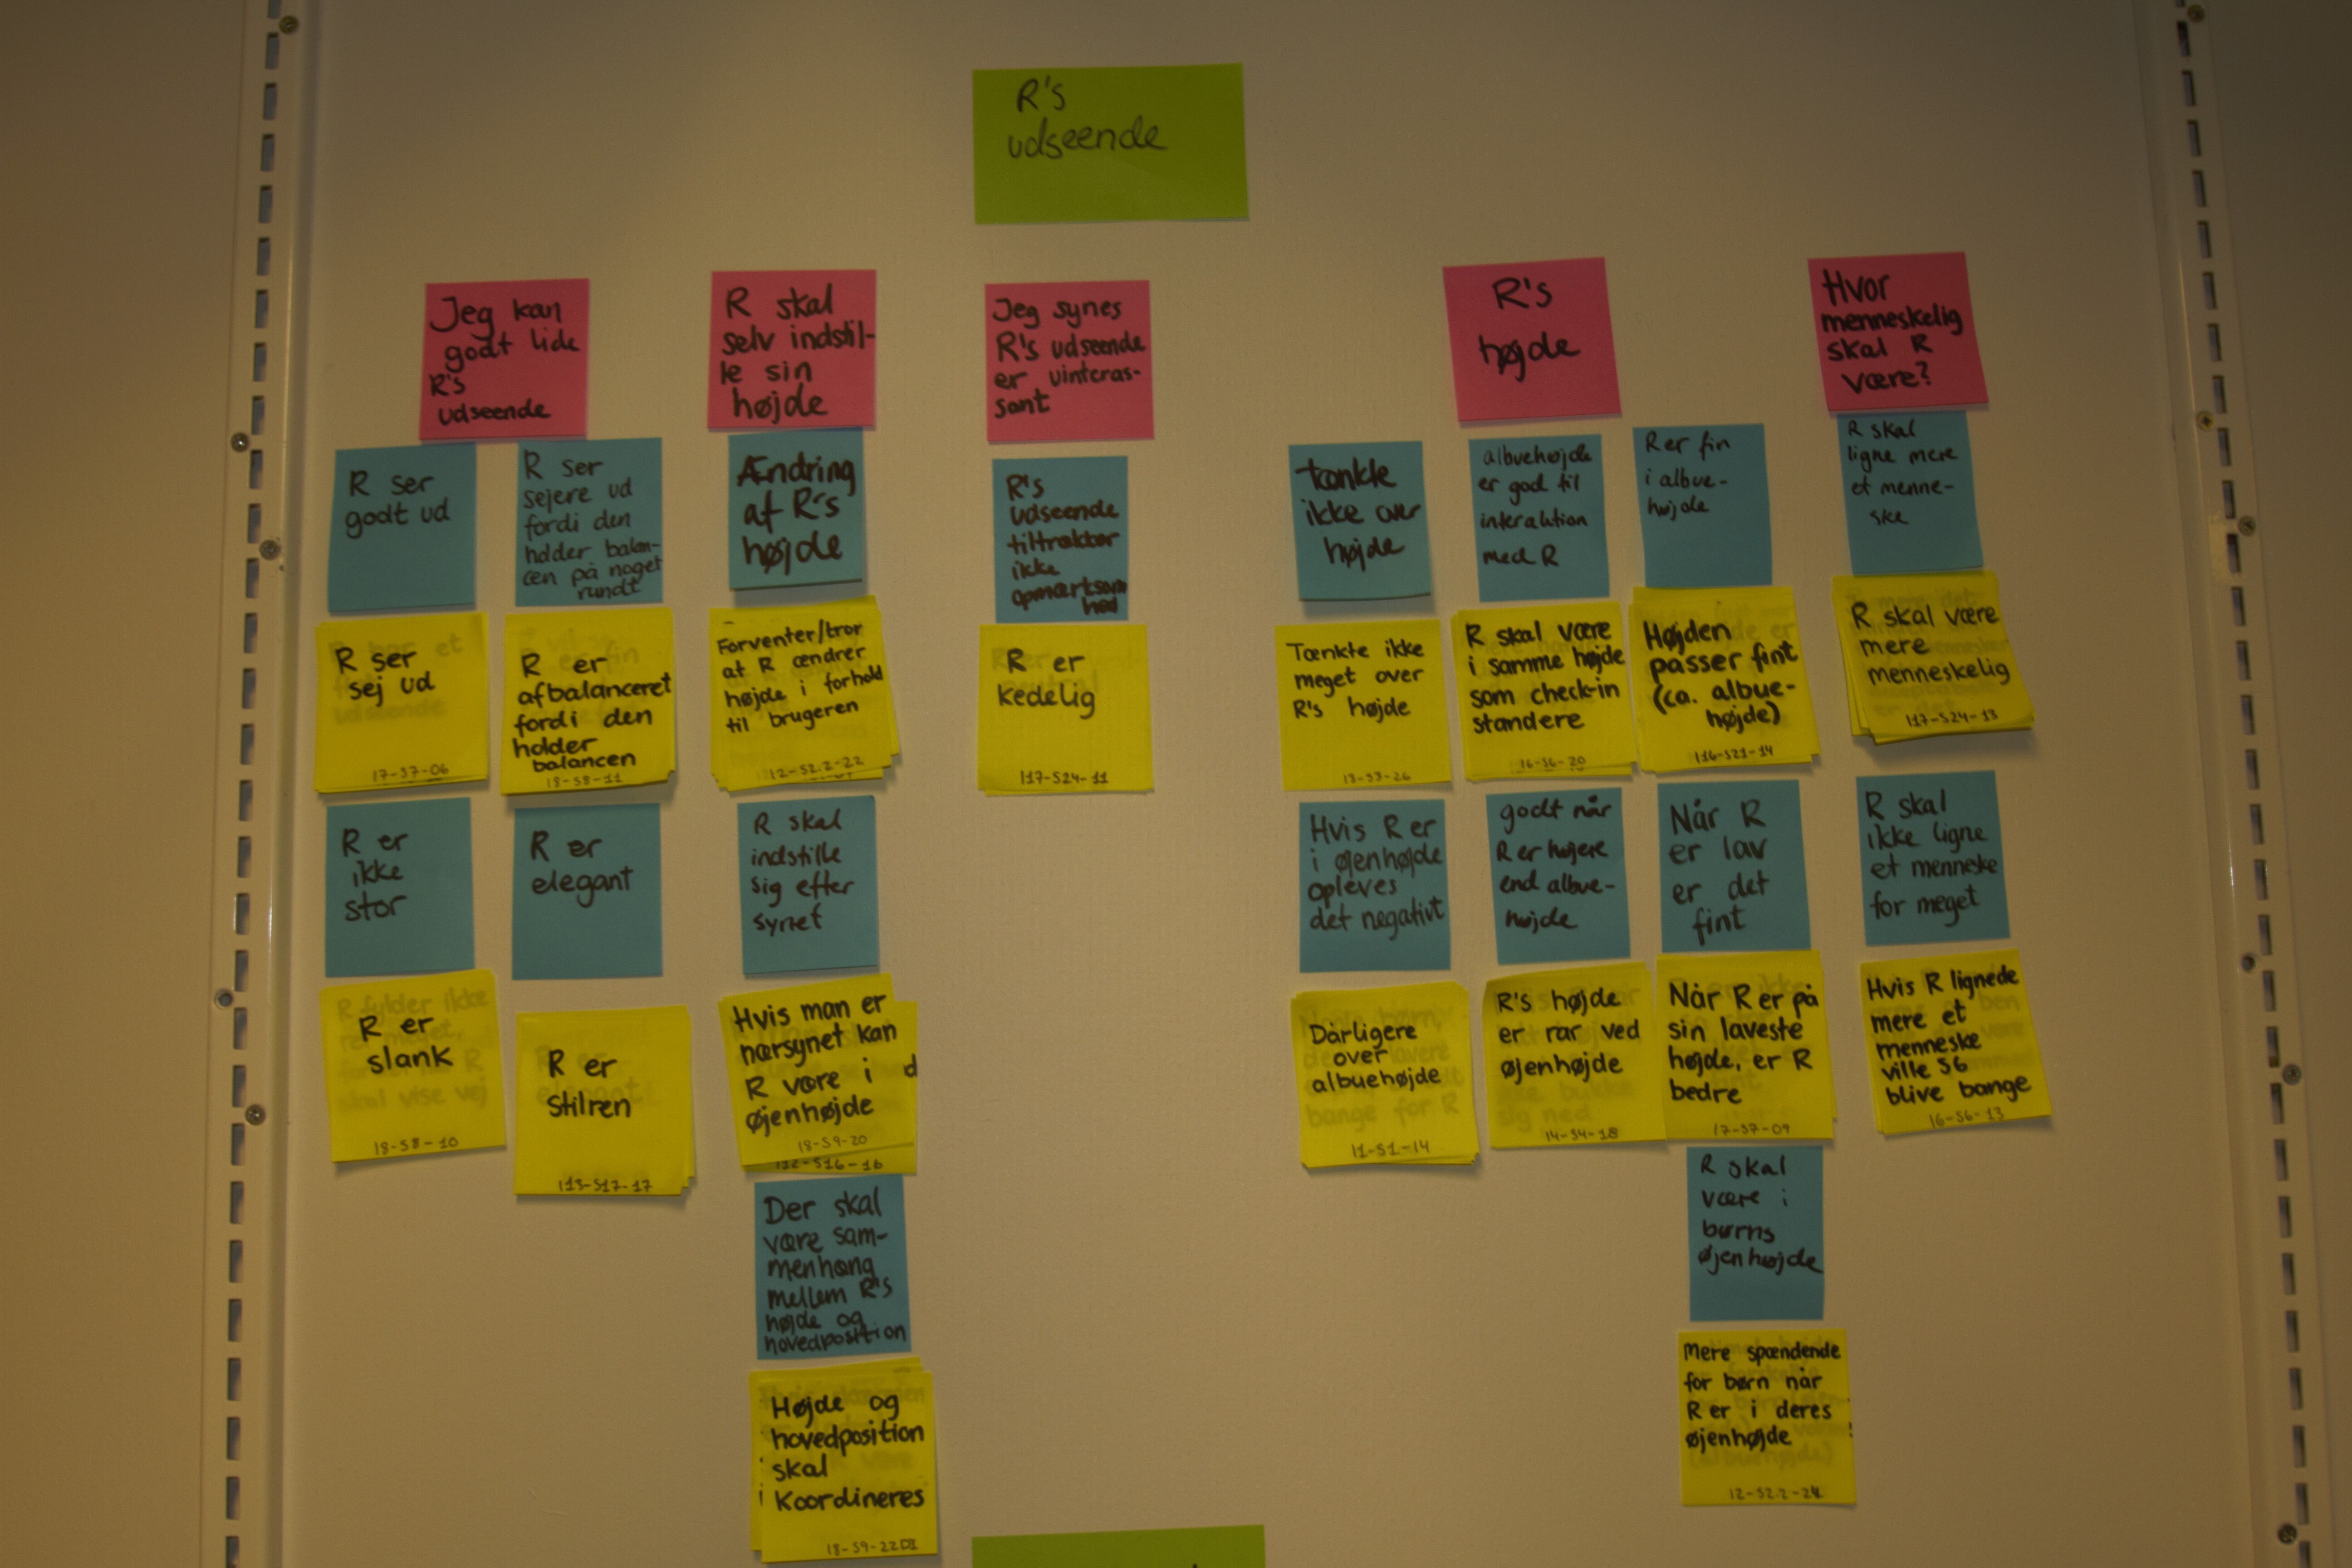
\includegraphics[width = 0.9\textwidth]{Figure/RsUdseende} 
\caption{Udsnit af det samlede \textit{affinity diagram}, som vedrører robottens udseende.}
\label{fig:RsUdseende}
\end{figure}
\noindent
%
Da dette miniprojekt bygger på data indsamlede i forbindelse med semesterprojektet er det ikke alle kategorier, der er angivet med pink labels, som har relevans for miniprojektet. I henhold til miniprojektet er det kun to af de pink labels, som kan anses for at være objektive attributter: \textit{R's højde} samt \textit{Hvor menneskelig skal R være?}, hvor R er en forkortelse for robot. I begge tilfælde er det muligt at ændre robottens fysiske karakteristika i forhold til højde og hvor menneskelig robotten perciperes. 
%
\begin{figure}[H]
\centering
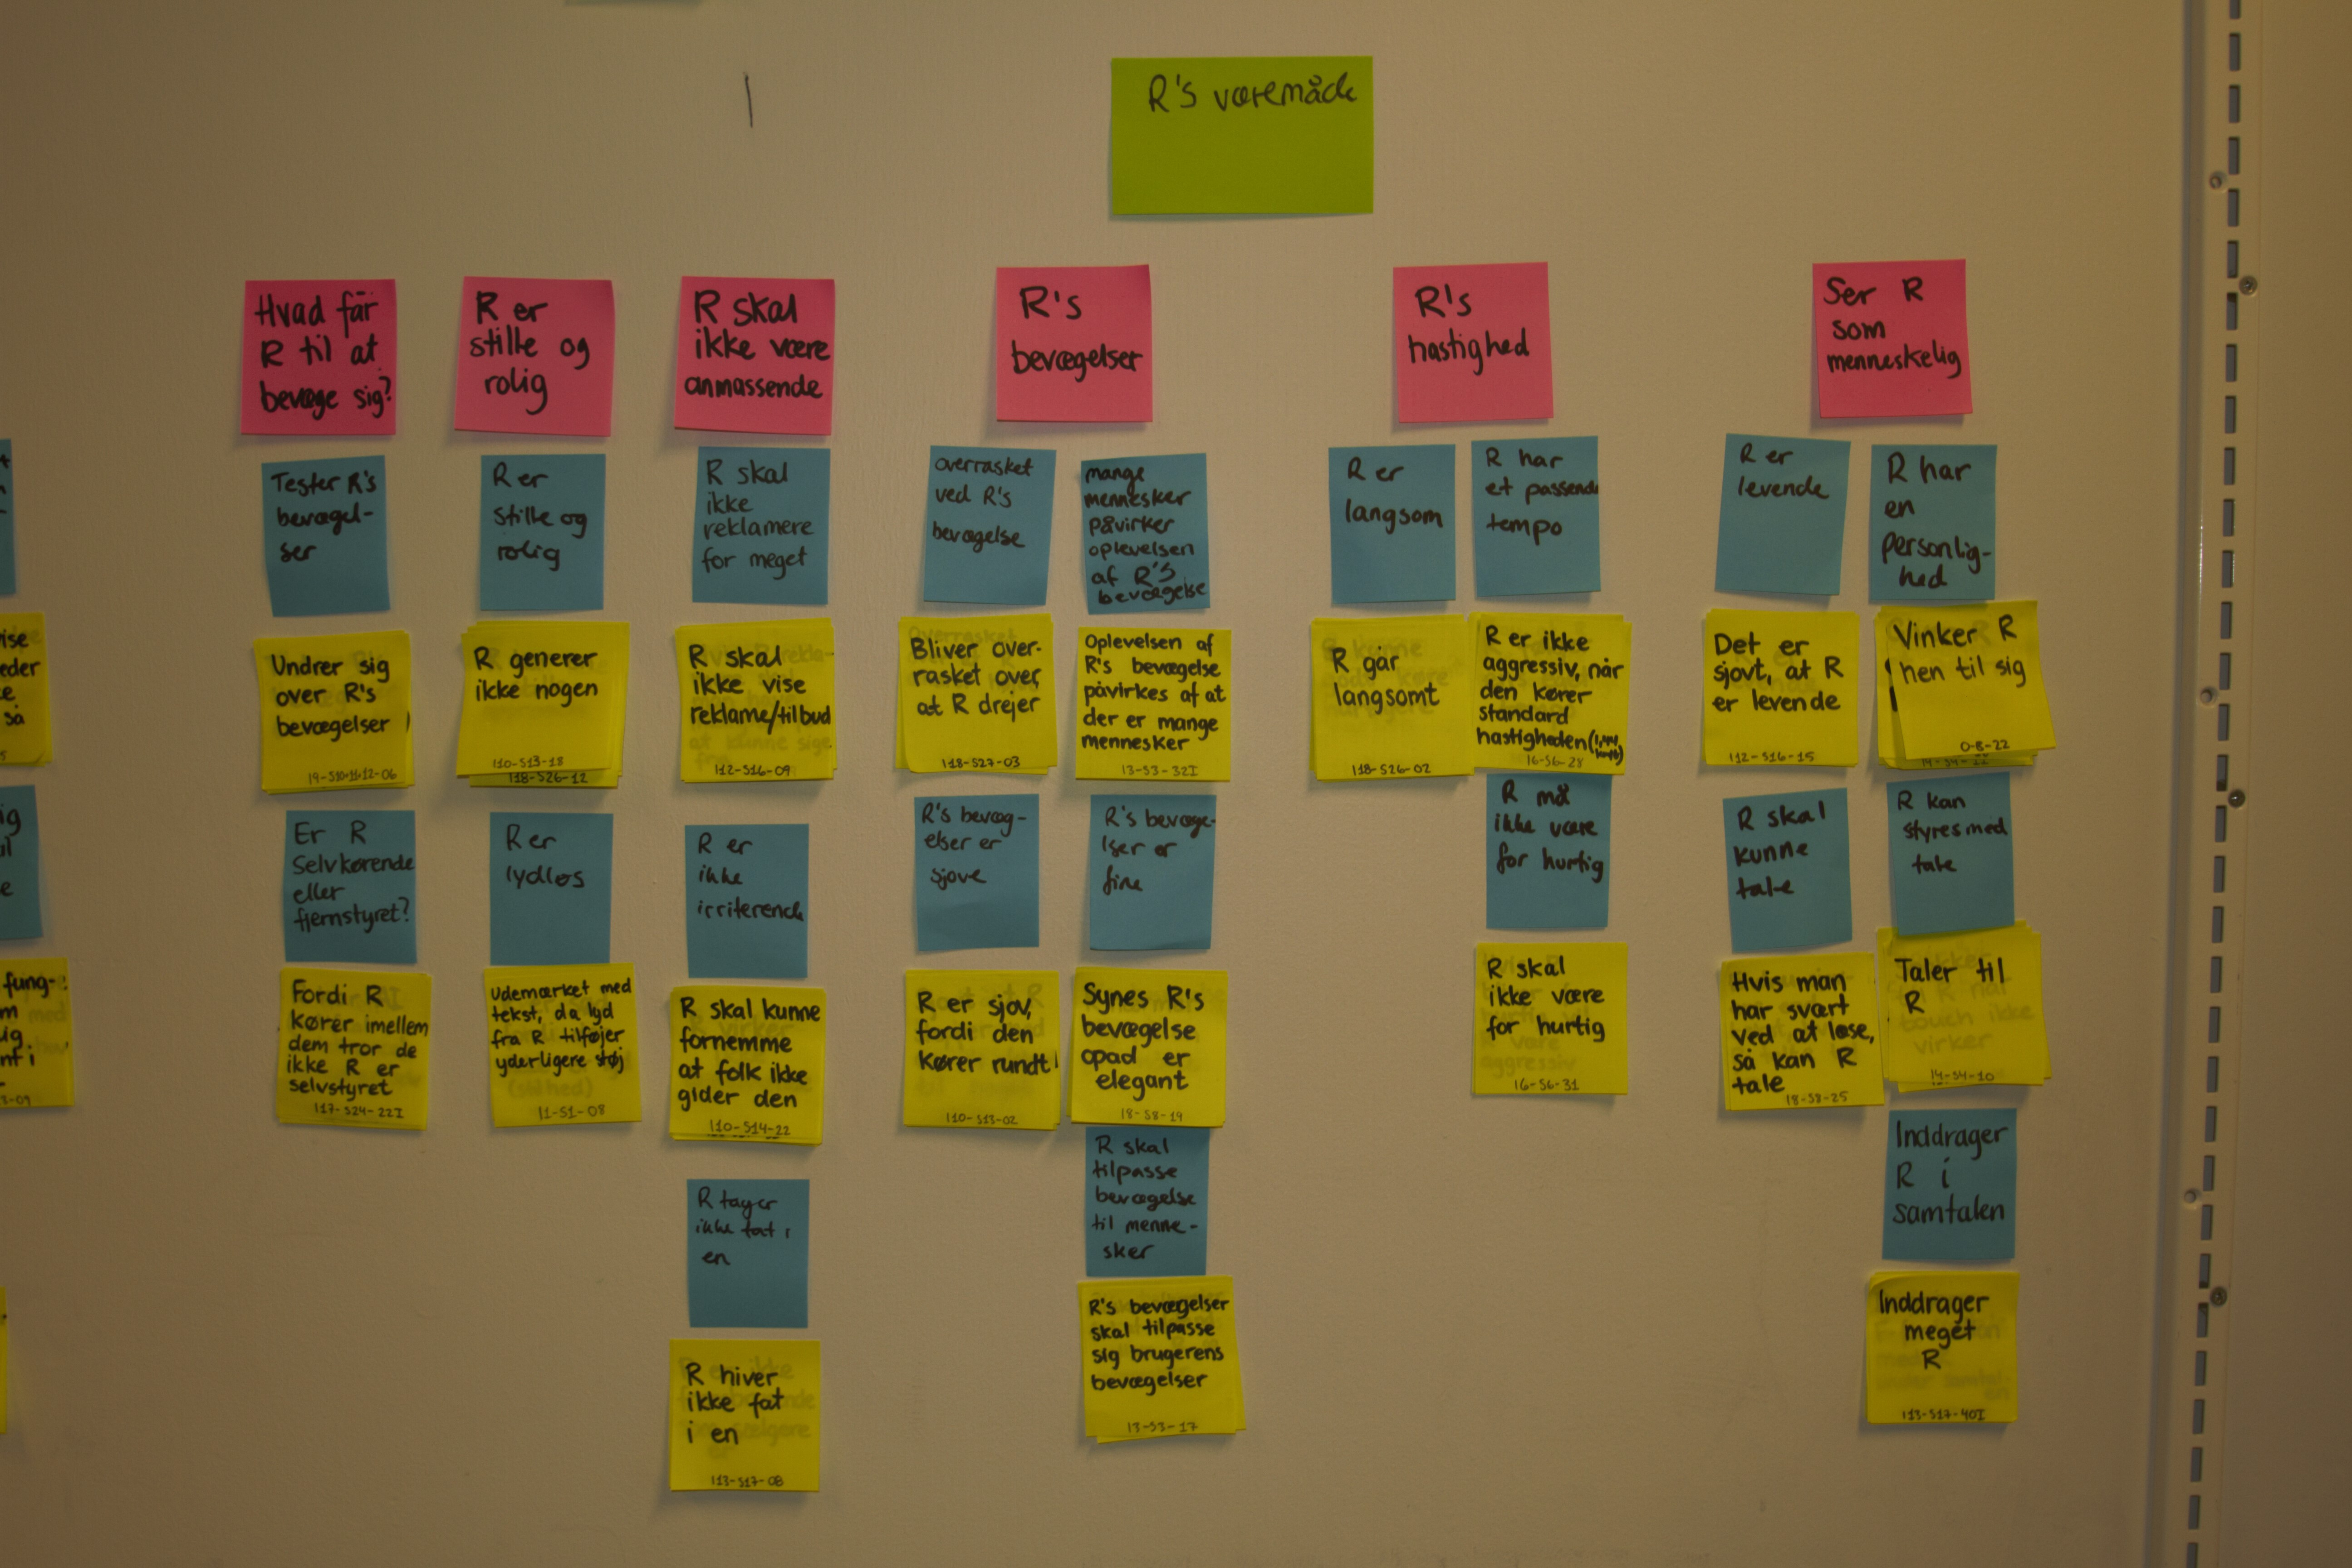
\includegraphics[width = 0.9\textwidth]{Figure/RsVaeremaade} 
\caption{Udsnit af det samlede \textit{affinity diagram}, som vedrører robottens væremåde.}
\label{fig:RsVaeremaade}
\end{figure}
\noindent
%



(beskriv her hvad vi så gjorde derefter.)

z